\chapter{Conclusion}
\label{sec:Conclusion}

%1. Results and success

%2. Why hard for others

%3. Essence of innovation
\section{Key Results}
\label{sec:keyResults}
In this thesis, five feature extraction algorithms have been compared using images captured by a Nao humanoid robot. A novel scoring function termed the \textit{Multi-Image Score} (MIS) has been developed in order to determine the optimal parameters for each  of the BRISK-based feature extraction algorithms.\\

Using these parameters, it was found that BRISK0 - U-BRISK generated the best overall performance. In the best case, this algorithm can match $90\%$ of the overlapping image pairs whilst maintaining a FP rate of $0$. This algorithm is also computationally efficient with a mean overall time of $8.8 ms$ in the best case which is well within the computational requirements of the Nao. BRISK0 - U-BRISK can therefore be implemented on the Nao. This algorithm can still work under varying illumination and can match overlapping images captured from different sensors albeit with decreased matching performance.\\

Another key result is that this algorithm can match Nao images with overlapping Google Street View images. The performance is reduced to a $TP_{FP=0}^{max}$ rate of $39\%$ but nevertheless can match overlapping image pairs. This can potentially be extended and improved to enable the Nao to perform street navigation.\\

Novel angle and distance constraints have been developed to remove invalid matches. A new interest point property entitled the mean response difference $\bar{dR}$ has been developed and can potentially become an additional constraint used to remove invalid matches.\\

Finally, a novel addition to the \textit{Augmented Monte Carlo Particle Filter} has been proposed. This will incorporate the feature extraction algorithm to enable the Nao to localise on the Robocup field.\\



\section{Problems and Limitations}
\label{sec:problemsLimitations}
%Problems and Limitations
The MPS parameters are calculated by averaging the maximum parameter settings for each dataset as discussed in \secref{sec:optimalParameters}. Averaging is sensitive to outliers and therefore taking the median value may improve the performance.\\

Due to the weak non-maximal suppression criteria imposed on the BRISK0 - U-BRISK algorithm, weak interest points are detected.  As a result of this relaxed constraint, a number of interest points may match that are not necessarily valid matches. An example of this can be seen in \figref{fig:weak}. A number of interest points in the left image are matched to an incorrect location in the right image having already passed the angle and distance constraints. This may imply that Radius Matching is not the best matching technique and 2-NN Matching should be used to increase the chances of removing these matches.\\

\begin{figure}
  \centering
    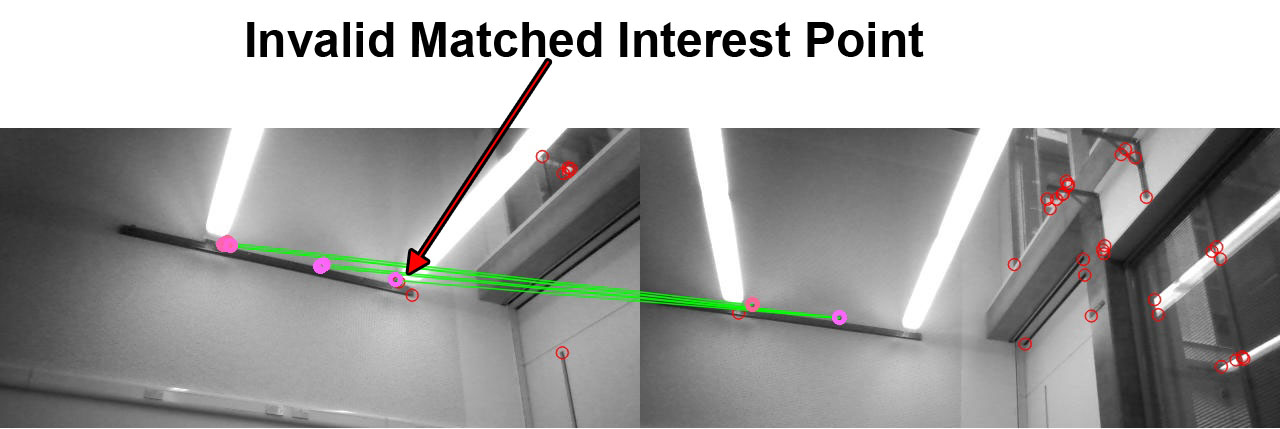
\includegraphics[width=1.0\textwidth]{../Drawings/Matching/dataset_valid_invalid_matches_photo.jpg}
    \caption{Invalid matches that have passed through the matching constraints} 
    \label{fig:weak}
\end{figure}

BRISK0 - U-BRISK is rotation variant which may prevent interest points from matching if either of the image pair undergo a significant rotation. To illustrate this, an identical image was  rotated clockwise by approximately $45^{\circ}$ and compared with its original version as shown in \figref{fig:rotationUbrisk}. An interest point has been identified between both of the fluorescent lights in each image but the interest point has not been matched due to this rotation. However, since the Nao will not be subject to rotations of this magnitude when coming onto the pitch after serving a penalty ban in the Robocup environment, this method is still a feasible option for Robocup. \\

\begin{figure}
  \centering
    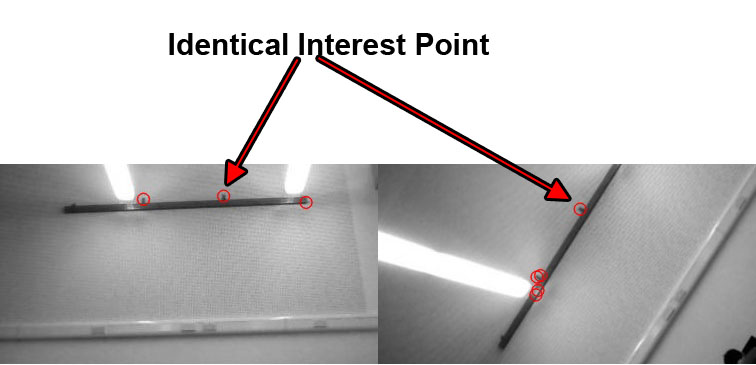
\includegraphics[width=1.0\textwidth]{../Drawings/Matching/rotationsUBRISK_photo.jpg}
    \caption{Matches lost due to BRISK0 - U-BRISK being rotation variant} 
    \label{fig:rotationUbrisk}
\end{figure}

A major problem that hinders all of the feature extraction algorithms are environments with many similar features. An example of this can be seen in the Google Street View Datasets. Both sides of the street contain buildings with similar looking windows as seen in \figref{fig:similarScene}. The left image has been captured with the Nao's camera and the right image is from Google Street View. Both images are from opposite sides of the street but contain similar features causing incorrect matches to be found.\\

\begin{figure}
  \centering
    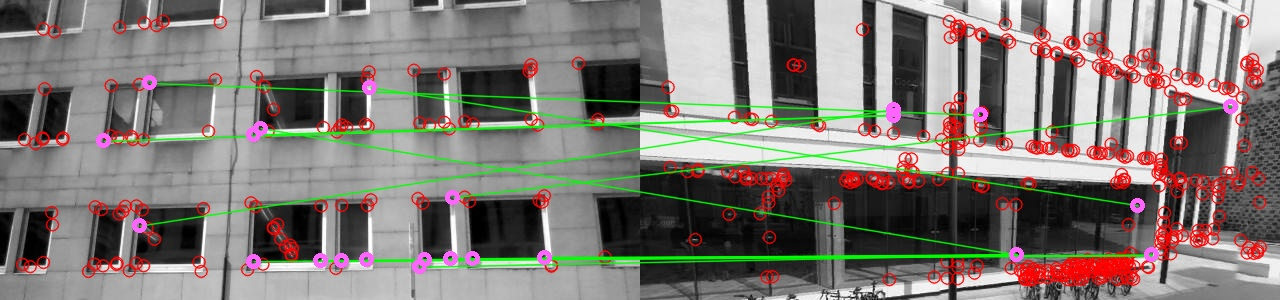
\includegraphics[width=1.0\textwidth]{../Drawings/Matching/dataset_similar_scene.jpg}
    \caption{Similar scenes cause ambiguities} 
    \label{fig:similarScene}
\end{figure}


BRISK0 - U-BRISK was analysed further and it was found that varying the illumination of an environment causes less valid interest point matches to be detected. However, BRISK0 - U-BRISK still detects on average $9.53$ valid matches for overlapping images in the worst case scenario. BRISK0 - U-BRISK is also sensitive to different camera settings and it has been found that matching image pairs from different cameras decreases the performance.\\

%Computing the median rather than the max - Outliers

%Learning distances to features using vision papers - see email

%Valid Matches - Overlapping images tend to produce a large number of matches that are invalid. However, since the images are similar and weak interest points are being detected, it seems plausible that matches will be generated in the same region and all other matches will be filtered out from the constraints. This is because the overlapping regions tend to have similar features???

%2-NN Constraints

%Similar looking scenes are going to cause a large number of ambiguous matches and reduce the performance.

%Recommendations for future work
\section{Recommendations for Future Work}
\label{sec:recommend}
The \textit{Multi-Image Score}(MIS) currently uses a grid search to find the optimal parameters. It has been shown that a random search can find parameters more efficiently than a grid search and this may enable more optimal parameters to be found at a lower computational cost \citep{Bergstra2012}.\\

BRISK0 - U-BRISK is currently rotation variant and this may cause problems outside of the Robocup environment if the Nao is subject to large rotations. Thus enforcing rotation invariance and optimising the algorithm differently may create more robust matching performance. This includes using a reduced sampling pattern as suggest in \citep{Leutenegger2011}. It may also be feasible to reduce the dimensionality of the bit vector by performing less intensity comparisons. \\

It may also be possible to utilise the order of the features in the BRISK-based techniques to yield better matching of overlapping image pairs. Previous work has been done using scanlines and 1D panoramas to match features using a dynamic programming algorithm \citep{Birchfield1998, Way1996, Briggs} and it may be possible to extend this algorithm to the 2D case.\\

It may also be useful to explore other types of feature extraction algorithms such as using vector quantisation histograms to represent features. This has been applied using SIFT and is entitled VQ-SIFT \citep{Chen2011}.\\

The localisation algorithm should also be implemented on the Nao robot incorporating BRISK0 - U-BRISK for the purposes of Robocup and this should be tested in real-time. In addition, the localisation algorithm is limited to the Robocup domain. This could be extended to a more general domain by calculating the distance to visual landmarks. One possible solution is to utilise a \textit{Markov Random Field} to estimate detailed 3D structure using a single image \citep{Saxena}. It may also be possible to calculate the bearing to the visual landmarks. \\ 

More extensive analysis needs to be performed on matching Nao images with Google Street View images to determine further improvements that need to be made to the algorithm in order to increase matching accuracy. It would also be interesting to test the other feature extraction algorithms on Google Street View images and compare their respective performance.\\